\documentclass[11pt, letterpaper]{report}
\usepackage[utf8]{inputenc}
\usepackage[T1]{fontenc}
\usepackage{helvet}
\renewcommand{\familydefault}{\sfdefault}
\usepackage{graphicx}
\usepackage{lipsum}
\usepackage[top=1in, bottom=1in, left=1in, right=1in]{geometry}
\usepackage{fancyhdr}
\usepackage{tocloft}
\usepackage{caption}
\captionsetup[figure]{labelfont={bf},name={Figure},labelsep=period, font={it}}
\usepackage{xltabular}
\usepackage{titlesec}
\titleformat{\chapter}[hang] 
{\normalfont\huge\bfseries}{}{1em}{} 
\titlespacing*{\chapter}{0pt}{0pt}{40pt}

\begin{document}
% Cover page
\newgeometry{top=2in, bottom=2in, left=2in, right=2in}
\begin{titlepage}
    \centering
    
\includegraphics[width=\textwidth]{images/logo.png}\par
    \vspace{1cm}
    {\bfseries SE 463: Software Requirements: Specification \& Analysis: \par}
    \vspace{0.5cm}
    {Daniel Berry \par}
    \vspace{5cm}
    {Group 01: \par}
    {Nishesh Jagga \par}
    {20741914 \par}
    \vspace{5cm}
    {Friday, July 14, 2023 \par}
\end{titlepage}
\restoregeometry

% Table of Contents
\tableofcontents
\thispagestyle{empty}
\clearpage

% Custom header and footer
\pagestyle{fancy}
\fancyhf{}
\rfoot{\thepage}
\lfoot{Deliverable 4}
\renewcommand{\headrulewidth}{0pt}

% Abstract
\chapter{Abstract}
\setcounter{page}{1}
A tool that aids a user in maintaining their budget by scheduling their weekly meals through suggesting recipes sourced from an online recipe database, that are suitable for their budget and align with their dietary restrictions. Following a personalization process, the users can expect to be presented with recipes that they might like to eat, made using ingredients that fit their budget, with prices from their local grocery store. To aid the grocery shopping process, any missing ingredients for the recipes in their planned meals would be added to a grocery list for the user to follow while shopping.

% Domain Model
\chapter{Domain Model}
\begin{figure}[h]
    \centering
    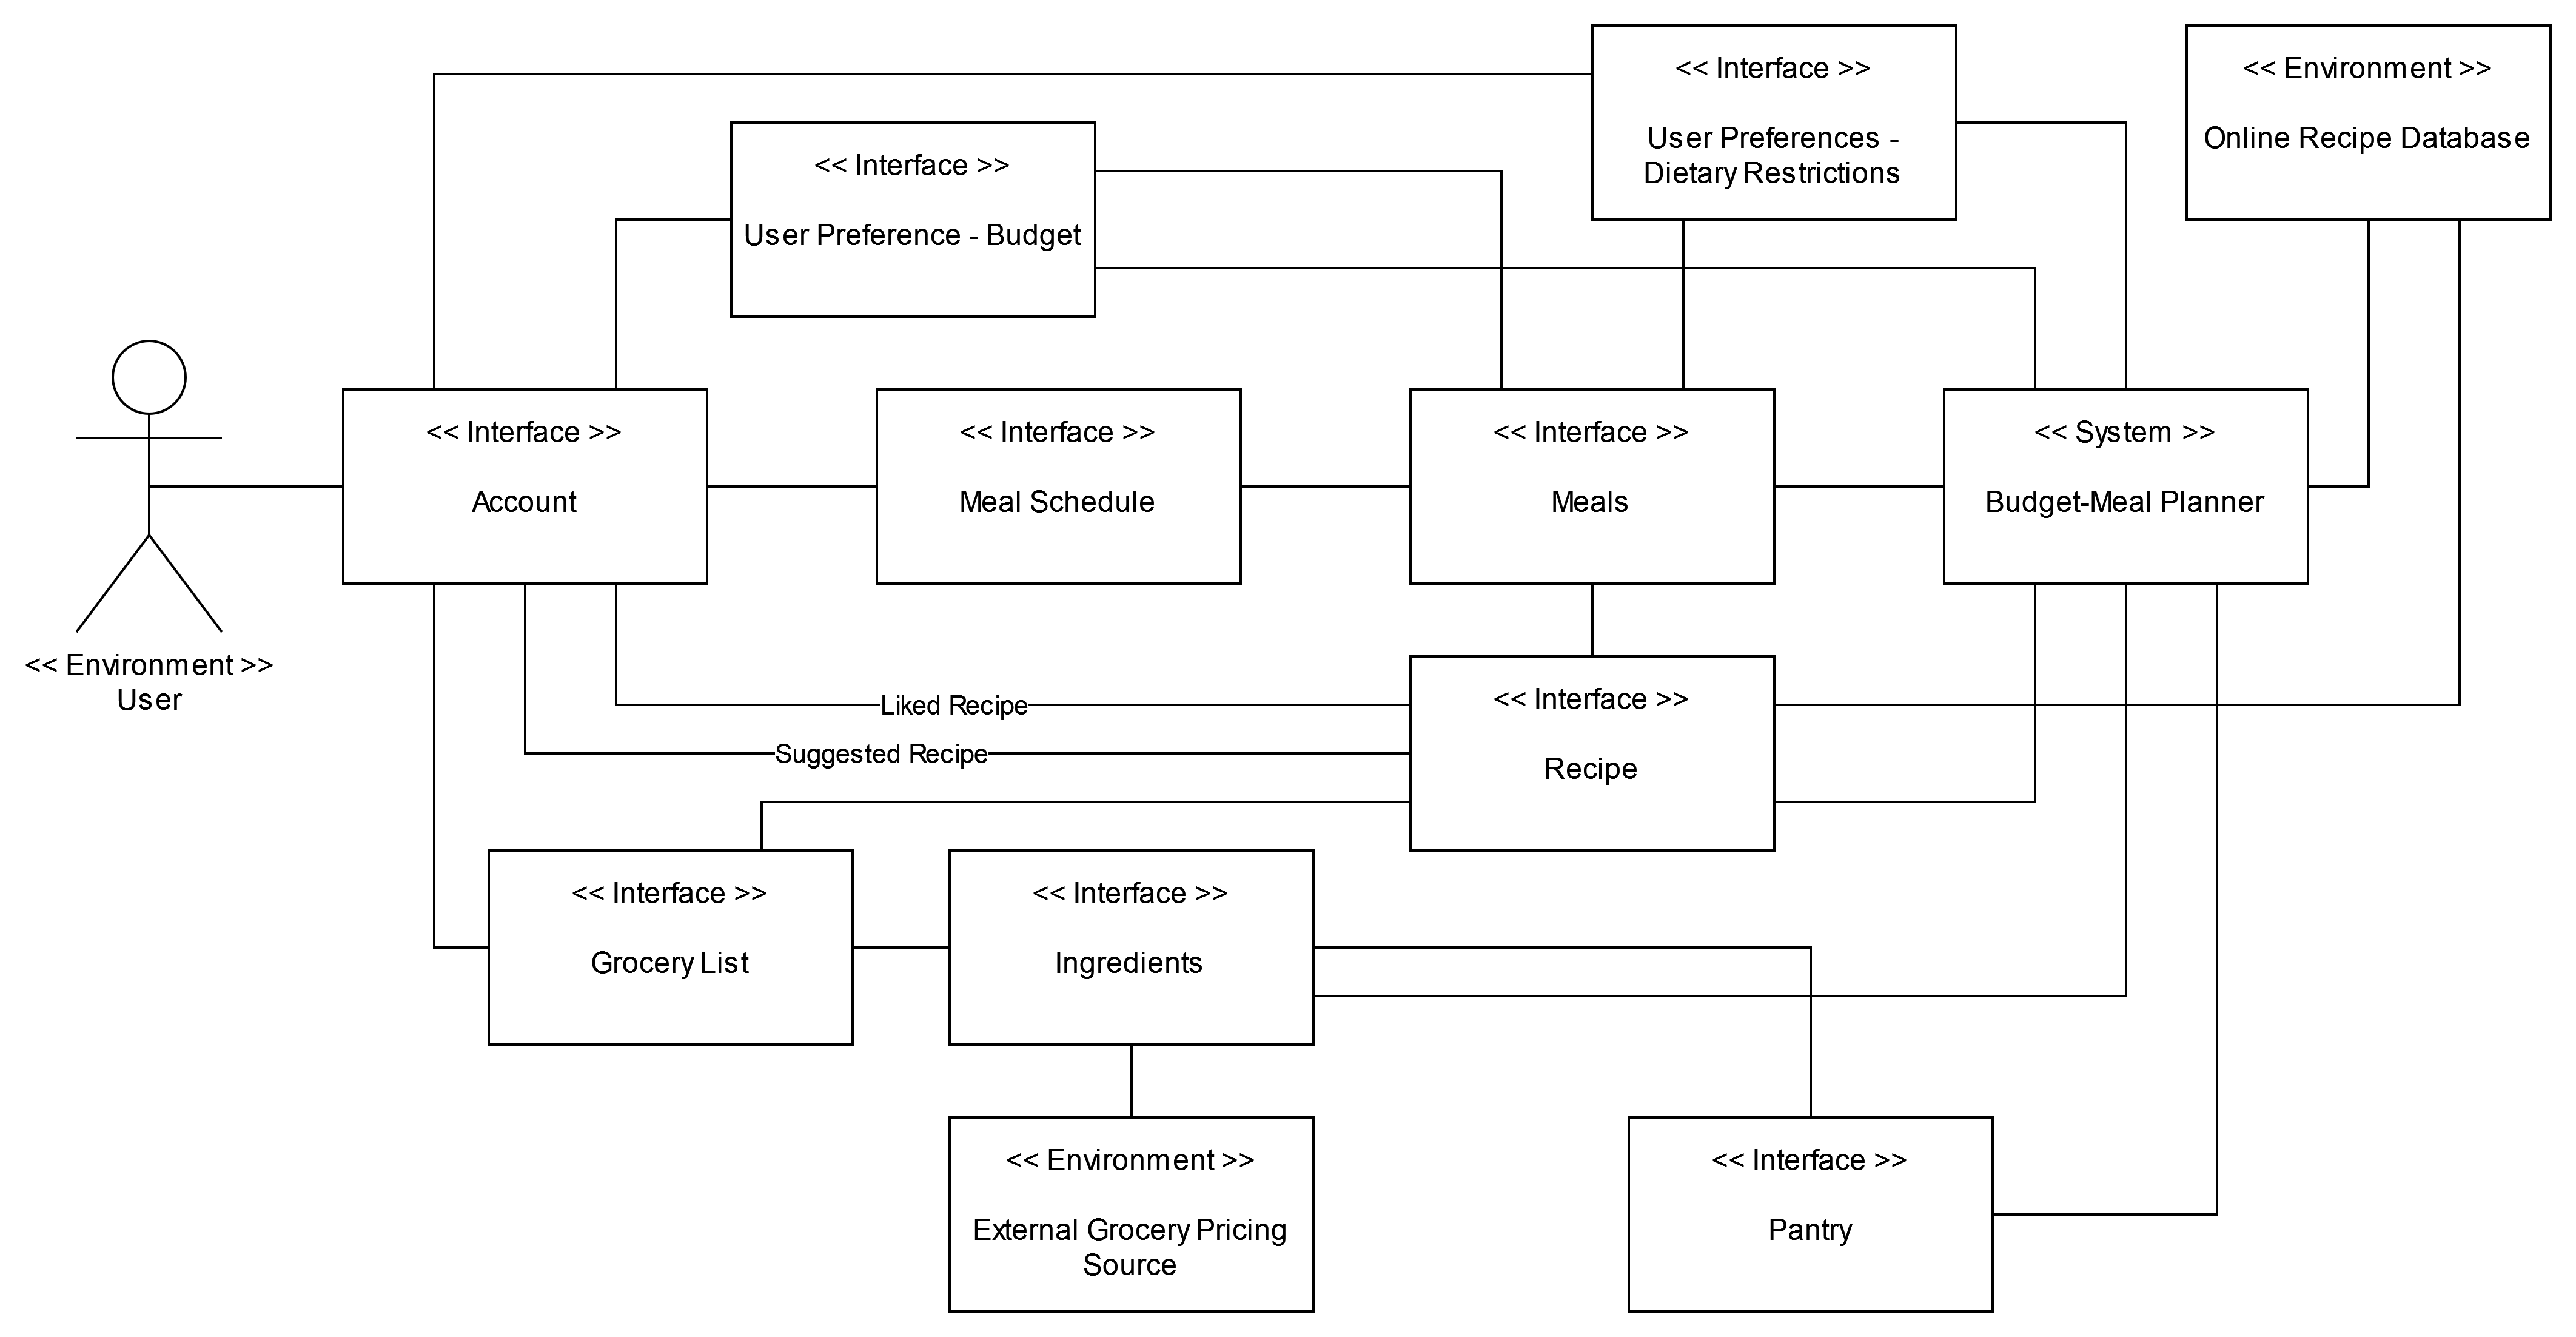
\includegraphics[width=\textwidth]{images/Domain_Model.png}
    \caption{Domain Model with World Diagram Superimposed}
\end{figure}

% Use Case Model
\chapter{Use Case Model}
\begin{figure}[h]
    \centering
    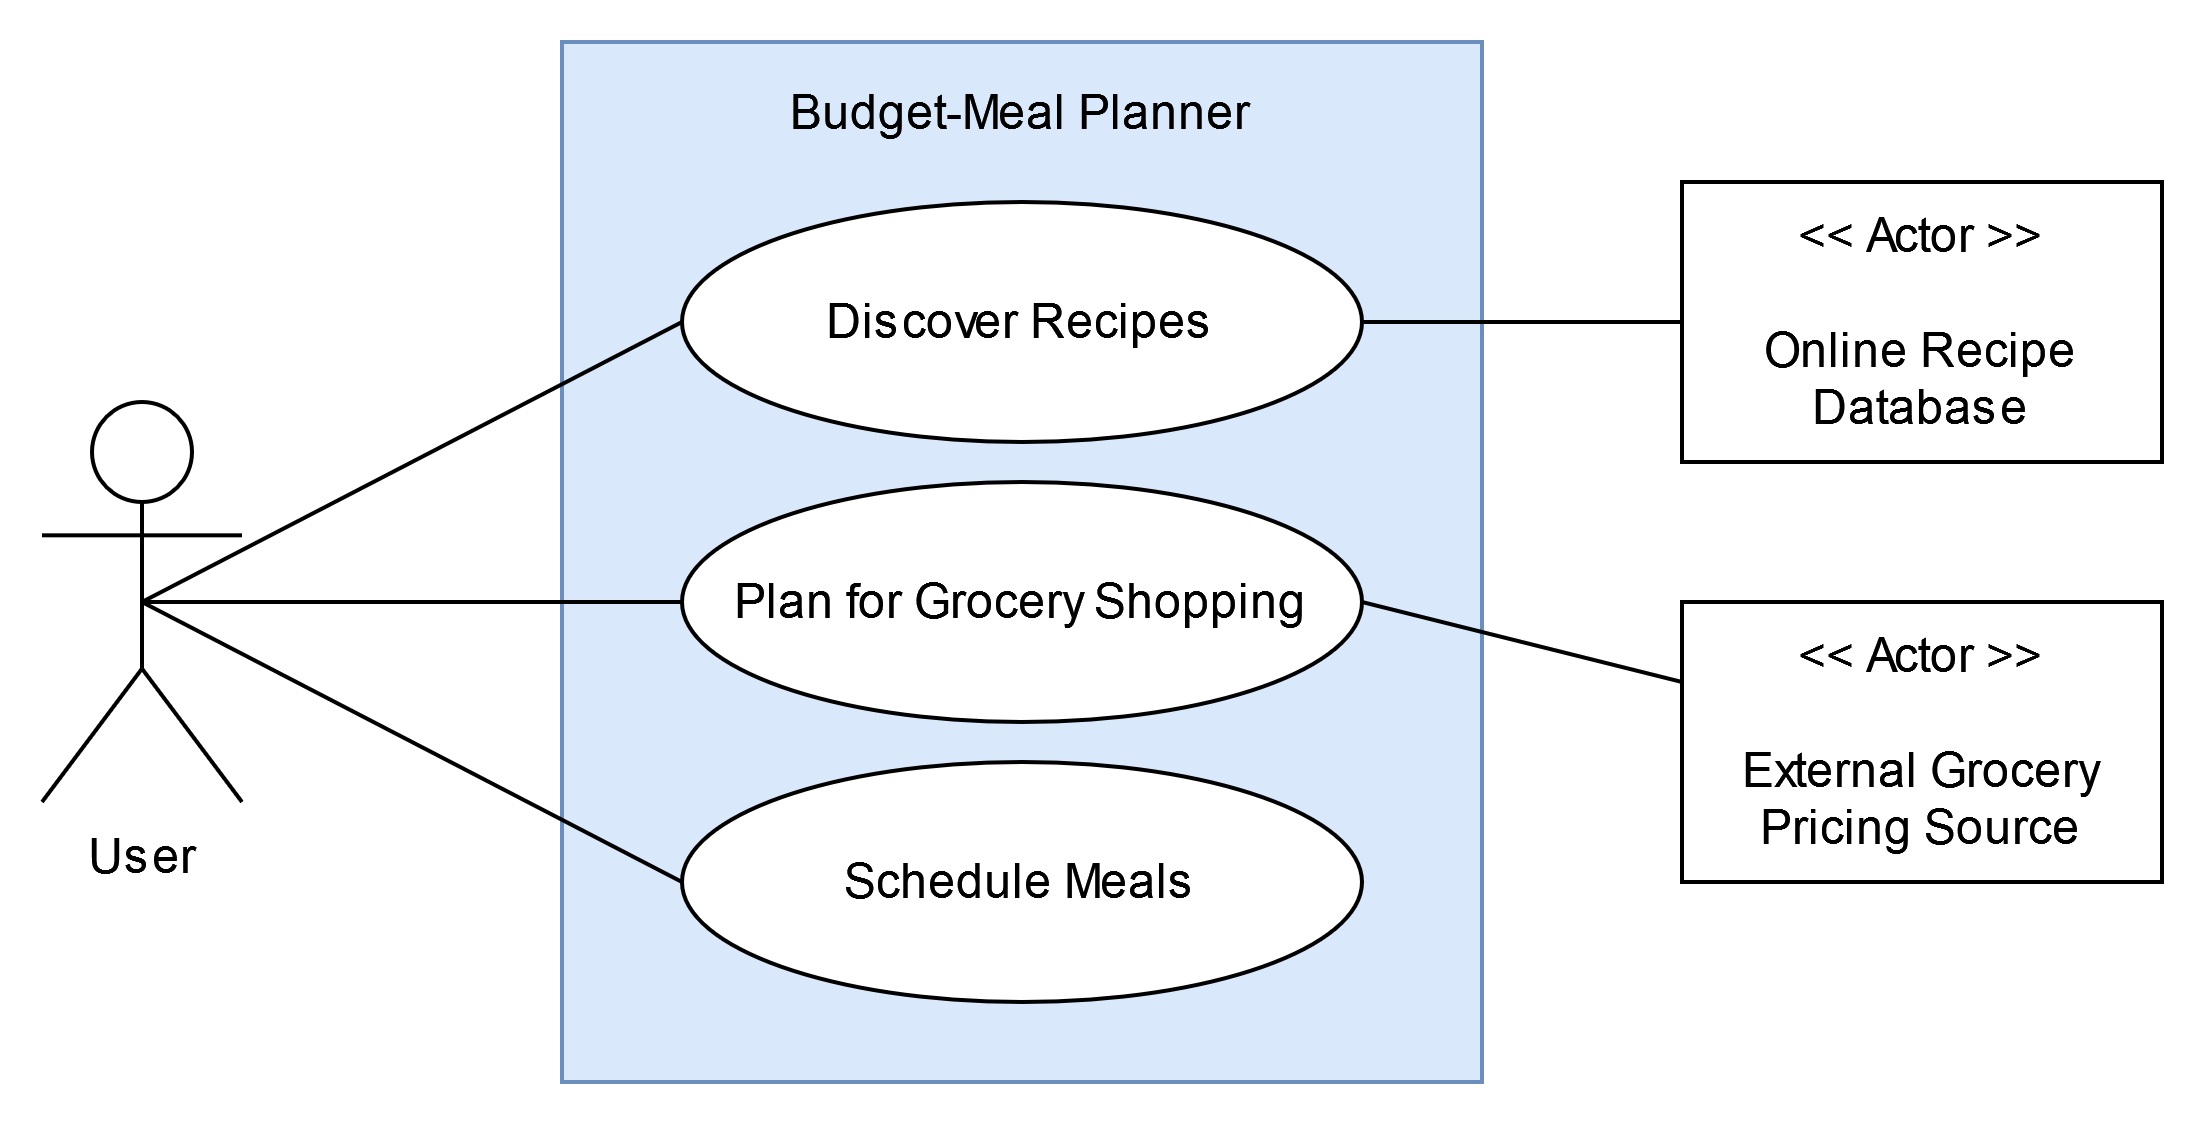
\includegraphics[width=\textwidth]{images/Use_Case.png}
    \caption{Use Case Model}
\end{figure}

\noindent \textbf{Discover Recipes}
\begin{itemize}
    \item Accept the users’ login credentials and open their account.
    \item Ask the user some questions to gather their preferences.
    \item Present the user with a list of recipes recommended for them.
    \item Accept a new recipe from the user and save it.
    \item Suggest alternative recipes, similar to the current recipe displayed.
    \item Hide a recipe from the user if they dislike it.
    \item Save a recipe to a “liked” collection for the user if they like it.
\end{itemize}
Domain Assumptions
\begin{itemize}
    \item The user has an account.
    \item Online Recipe Database is available.
    \item External Grocery Pricing Source is available.
    \item Recipe is valid, and can be cooked.
    \item The ingredients in the recipe are available in the External Grocery Pricing Source or the user’s pantry.
\end{itemize}

\noindent \textbf{Plan for Grocery Shopping}
\begin{itemize}
    \item Display the user’s current ingredient quantities in the pantry.
    \item Display the user’s grocery list.
    \item Add all ingredients from a recipe to the grocery list.
    \item Move ingredients from grocery list to pantry based on what the user bought from the grocery store.
\end{itemize}
Domain Assumptions
\begin{itemize}
    \item The user has an account.
    \item External Grocery Pricing Source is available.
    \item The currency of the External Grocery Pricing Source is the same as the user’s currency.
    \item The prices are up to date, and representative of the real world.
    \item 
\end{itemize}

\noindent \textbf{Schedule Meals}
\begin{itemize}
    \item Assign a recipe to a meal on a user’s schedule.
    \item Display a user’s meal plan (schedule).
\end{itemize}
Domain Assumptions
\begin{itemize}
    \item The user has an account.
    \item Recipes are accessible.
    \item There are enough recipes available to fill the user’s schedule.
    \item The ingredients for the meals are available in the user’s pantry, or can be procured.
\end{itemize}

% Scenarios
\chapter{Scenarios}
\noindent \textbf{UC 1: Discover Recipes} \\

\noindent \textbf{UC 2: Plan for Grocery Shopping} \\

\noindent \textbf{UC 3: Schedule Meals} \\

% User Stories
\chapter{User Stories}
\end{document}
